\documentclass[a4paper,12pt]{article}

\usepackage{textcomp}
\usepackage{amsmath, amssymb}
\usepackage{bm}
\usepackage{relsize}
\usepackage{parskip}
\usepackage{{../NotesTeX}}
\usepackage{pgfplots}
\usepackage{slashbox}
\everymath{\displaystyle}

\pgfplotsset{compat=1.18}

\DeclareMathOperator{\projection}{proj}
\newcommand{\dotp}[2]{\left\langle #1,#2 \right\rangle}
\newcommand{\proj}[2]{\projection_{#1}\left(#2\right)}
\newcommand{\C}{\mathcal{C}}

\title{Differential Geometry}
\date{\today}

\begin{document}
\maketitle

\part{Prerequisites}
\section{Matrices}
\begin{theorem}
	To prove a system of vectors $\{\va{u}_1,\va{u}_2,\ldots,\va{u}_n\} $ is free we prove:
	\[
		\det \mqty[\vline&\vline&\vline&&\vline\\\va{u}_1&\va{u}_2&\va{u}_3&\cdots&\va{u}_1\\\vline&\vline&\vline&&\vline] \neq  0
		.\]
\end{theorem}

\begin{theorem}
	A transition matrix $P_{B\to B'}$\marginnote{transition matrices are always square and invertible ($\det P \neq 0$)}between 2 basis $B=\{\va{u}_1,\va{u}_2,\va{u}_3\} $ and $B'=\{\va{v}_1,\va{v}_2,\va{v}_3\} $ we start by solving the system
	\[
		\mqty[\vline&\vline&\vline&&\vline\\\va{u}_1&\va{u}_2&\va{u}_3&\cdots&\va{u}_n\\\vline&\vline&\vline&&\vline] \mqty[\alpha_n\\\beta_n\\\gamma_n] = \mqty[\vline\\\va{v}_n\\\vline]
		.\]
	or in other words finding
	\[
		\begin{cases}
			\va{v}_1 & =\alpha_1\va{u}_1+\beta_1\va{u}_2+\gamma_1\va{u}_3 \\
			\va{v}_2 & =\alpha_2\va{u}_1+\beta_2\va{u}_2+\gamma_2\va{u}_3 \\
			\va{v}_3 & =\alpha_3\va{u}_1+\beta_3\va{u}_2+\gamma_3\va{u}_3 \\
		\end{cases}
		.\]
	Finally we say that
	\[
		P_{B\to B'} = \mqty[\alpha_1&\alpha_2&\alpha_3\\\beta_1&\beta_2&\beta_3\\\gamma_1&\gamma_2&\gamma_3]
		.\]
\end{theorem}
\begin{remark}
	To find the transition matrix in the inverse direction (from $B'$ to $B$ ) we simply do
	\[
		P_{B'\to B} = {P_{B\to B'}}^{-1}
		.\]
\end{remark}
\section{Vectors}
\begin{definition}
	We define an operation called the scalar product (dot product)
	\begin{align*}
		\dotp{\cdot}{\cdot}: \mathbb{R}^n \times \mathbb{R}^n & \longrightarrow \mathbb{R}                                     \\
		\va{u},\va{v}                                         & \longmapsto \dotp{\va{u}}{\va{v}} =\sum_{n=1}^{n} v_i\cdot u_i
		.\end{align*}
\end{definition}

\begin{definition}
	We define the usual norm on $\mathbb{R}$ to be
	\begin{align*}
		\|\cdot \|: \mathbb{R}^n & \longrightarrow \mathbb{R}                            \\
		\va{u}                   & \longmapsto \|\va{u}\| = \sqrt{\dotp{\va{u}}{\va{u}}}
		.\end{align*}
\end{definition}
\begin{theorem}
	The projection of a vector $\va{u}$ on to another vector $\va{v}$ is
	\[
		\proj{\va{v}}{\va{u}} = \frac{\dotp{\va{u}}{\va{v}}}{\|\va{v}\|^2}\va{v}
		.\]
\end{theorem}

\subsection{Gram–Schmidt process}
The aim of this process is to find a new basis $\Gamma=\{\vu{e}_1,\vu{e}_2,\ldots,\vu{e}_n\} $ derived from a basis $B=\{\va{v}_1,\va{v}_2,\ldots,\va{v}_n\} $ such that it is orthonormal or in other words
\[
	\forall \vu{x},\vu{y}\in \Gamma: \dotp{\vu{x}}{\vu{y}}=0 \qq{and} \|\vu{x}\|=1
	.\]
We find it as follows
\begin{align*}
	\va{u}_1 & = \va{v}_1 \quad                                                                                    & \vu{e}_1 = \frac{\va{u}_1}{\|\va{u}_1\|} \\
	\va{u}_2 & = \va{v}_2-\proj{\va{u}_1}{\va{v}_2}                                                                & \vu{e}_2 = \frac{\va{u}_2}{\|\va{u}_2\|} \\
	\va{u}_3 & = \va{v}_3-\proj{\va{u}_1}{\va{v}_3}-\proj{\va{u}_2}{\va{v}_3}                                      & \vu{e}_3 = \frac{\va{u}_3}{\|\va{u}_3\|} \\
	\vdots   &                                                                                                     &                                          \\
	\va{u}_n & = \va{v}_n-\proj{\va{u}_1}{\va{v}_n}-\proj{\va{u}_2}{\va{v}_n}-\ldots-\proj{\va{u}_{n-1}}{\va{v}_n} & \vu{e}_n= \frac{\va{u}_n}{\|\va{u}_n\|}  \\
\end{align*}

\part{Sequence of Functions}


\section{Introduction}

In previous courses, we analysed the convergence of sequences of numbers (example: $U_n = \left\{ \frac{1}{4},\frac{1}{9},\frac{1}{16},\ldots \right\} =\sum_{n=1}^{\infty} \frac{1}{n^2} $) with a series of tests. In this course we will be analysing sequences of \emph{functions} $f_n(x)$.\\
An example, is $f_n(x)=\frac{x}{x+n} =\{f_1,f_2,f_3,\ldots\}  =\left\{ \frac{x}{x+1},\frac{x}{x+2},\frac{x}{x+3},\ldots \right\}$.\\

There are 2 ways these sequences can converge: pointwise and uniformly

\begin{figure}[H]
    \centering
    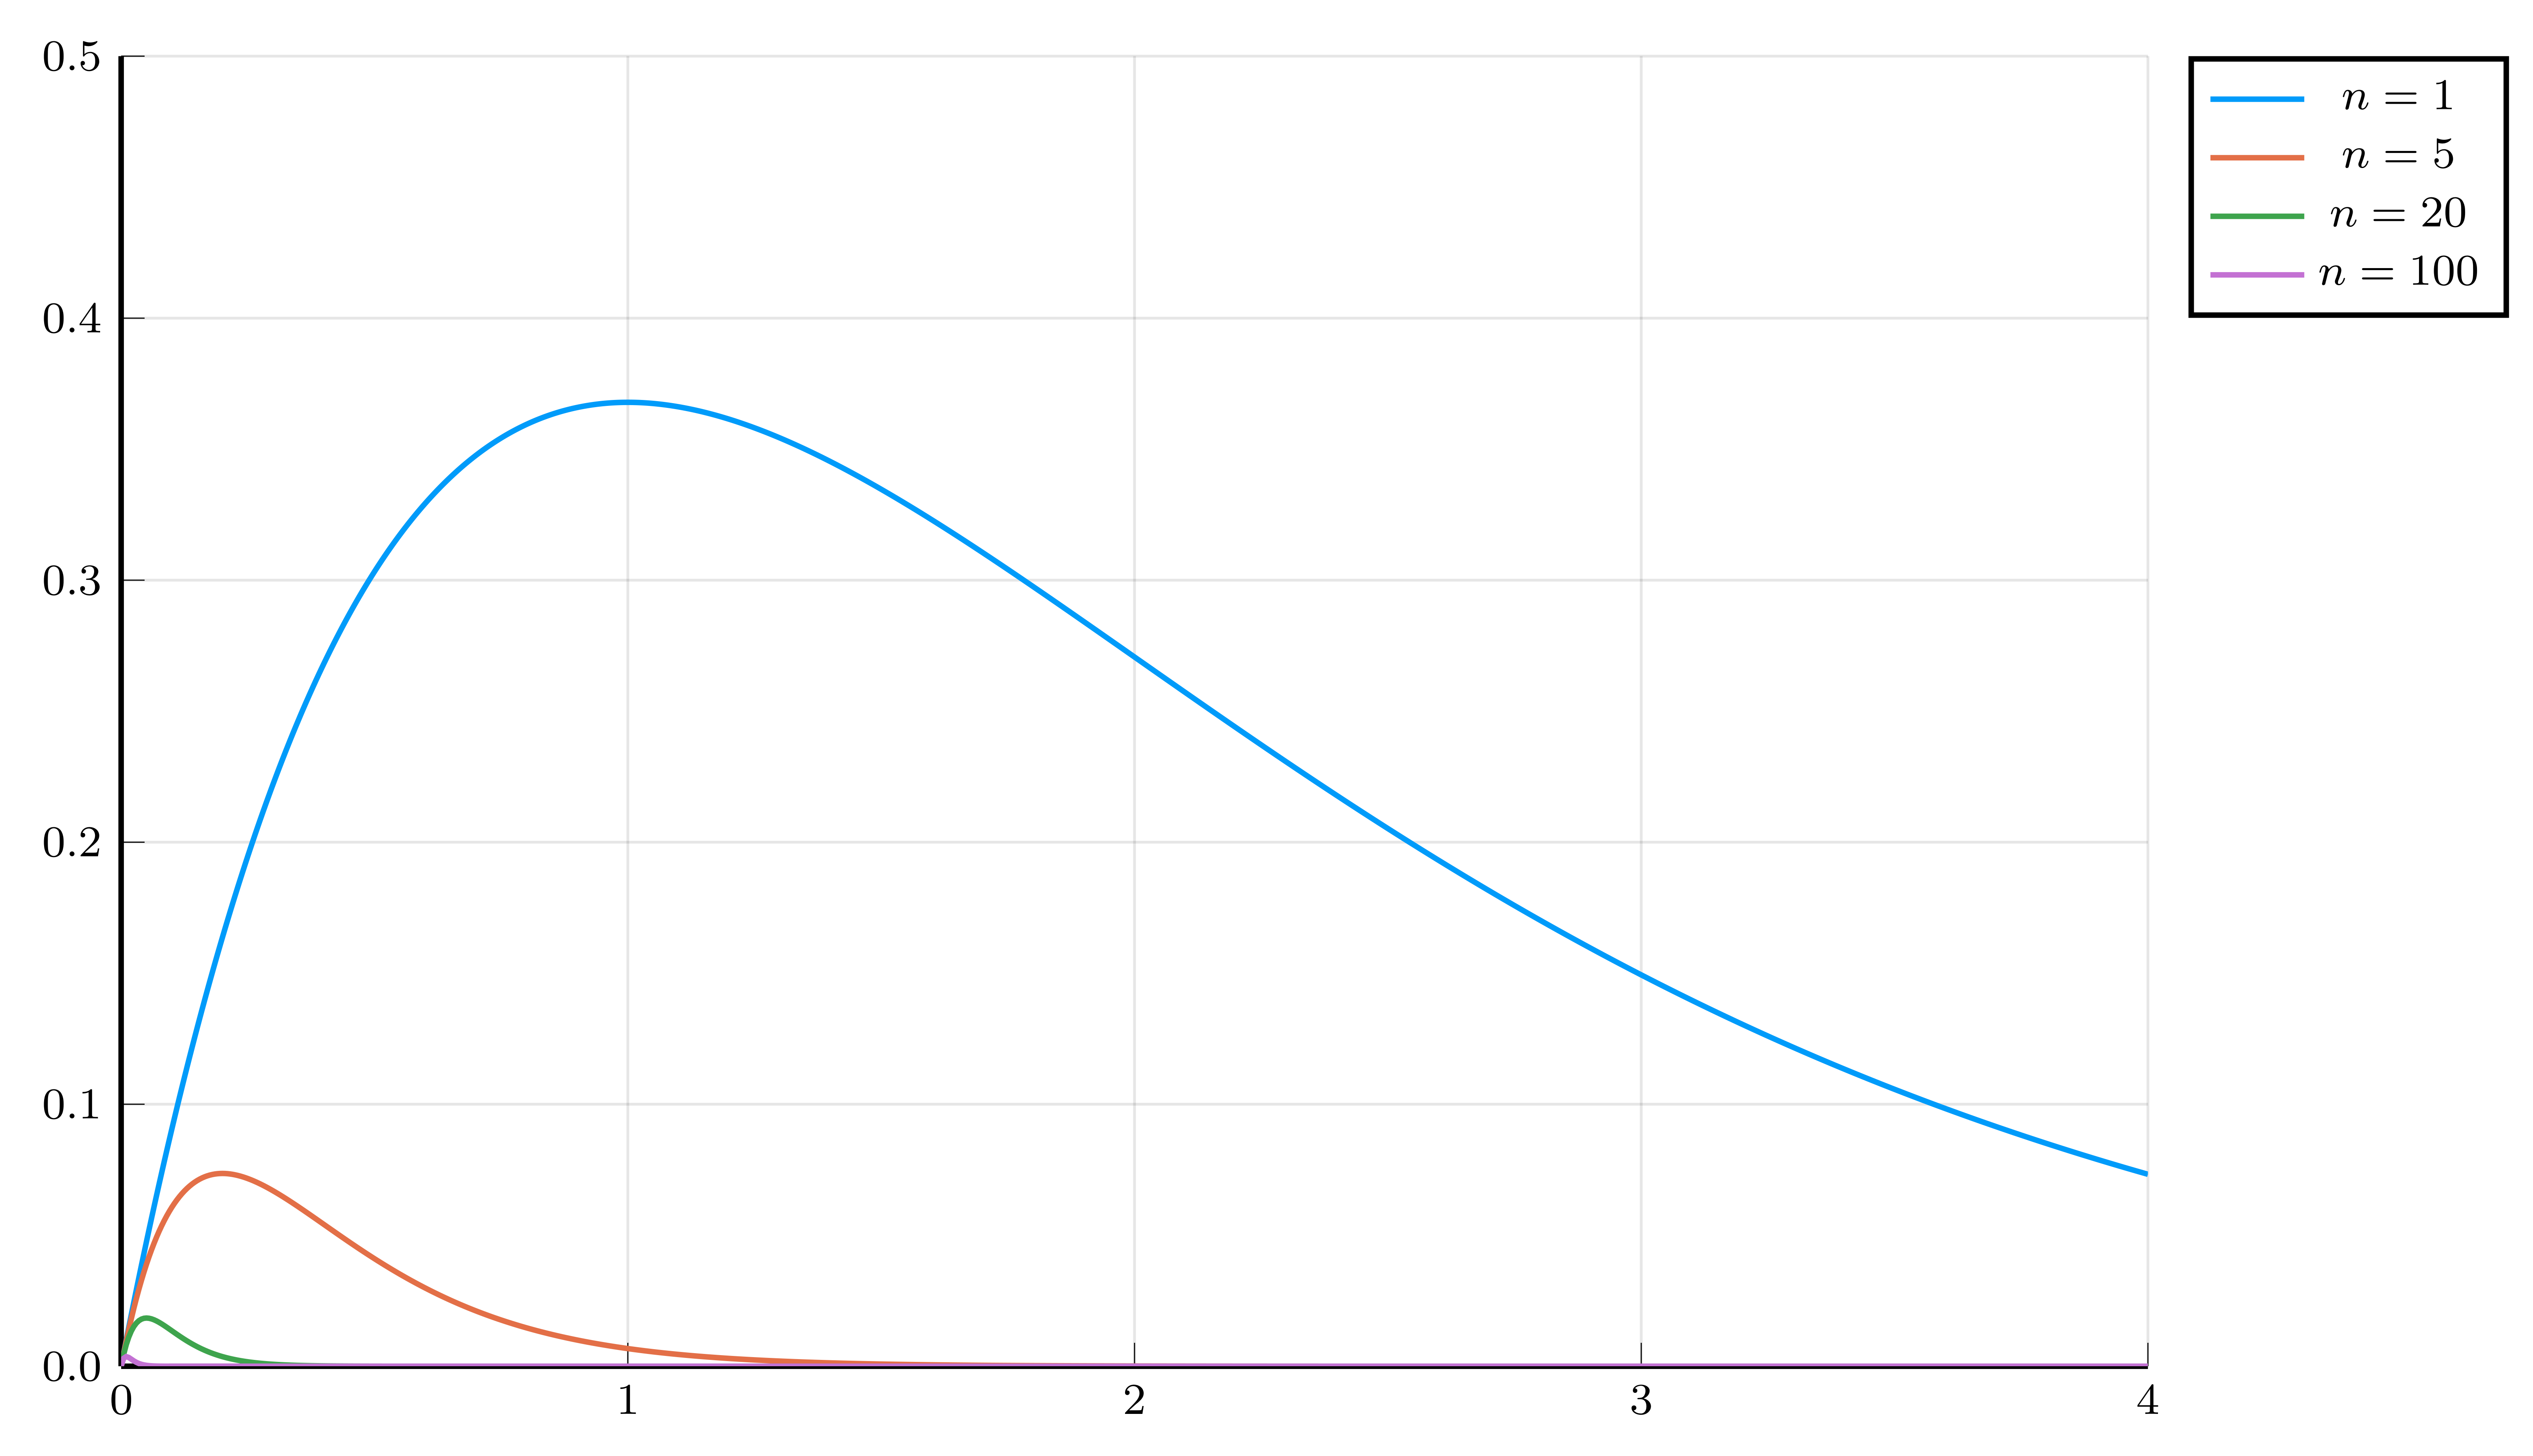
\includegraphics[width=\textwidth]{plot1.png}
    \caption*{Plot of the sequence $f_n(x)=xe^{-nx}$}
    \label{fig:plot}
\end{figure}

\section{Pointwise convergence}

This is a very natural way of proving convergence since all you have to do is fix $f_n$ to a point $x$ then the sequence just becomes an ordinary sequence of numbers, and if they all converge to a number we can define a limit function $f$ and say that they converge to $f$ pointwisely.

\begin{definition}
    We say that a sequence of functions $f_n$ where $f_n:I \to \mathbb{R},I\subset \mathbb{R}$, converges pointwise to function $f:I\to \mathbb{R}$ on the interval $I$ if:
    \[
    \forall x\in I \; \forall \epsilon >0 \; \exists n\in \mathbb{N} \; \forall n\ge \mathbb{N}: \quad \left| f_n(x)-f(x) \right|<\epsilon 
    .\] 
\end{definition}
You either prove convergence using the definition or by doing:
\begin{enumerate}
    \item Let $x=0$ then find $\lim_{n \to \infty} f_n(0)=$ some $f(x)$
    \item Then let $x\neq 0$ and again find $\lim_{n \to \infty} f_n(x)=f(x)$ 
    \item If neither of the results are unbounded $\pm \infty$ then we say $f_n(x)$ is convergent to some $f(x)$
\end{enumerate}

\begin{remark}
    if the result of step 1 is $g(x)$ and step 2 results in $h(x)$ where $g(x)\neq h(x)$ then we define the limit function:
     \[
         f(x)=\begin{cases}g(x)&x=0\\h(x)&x\in ]0,1]\end{cases}
    .\] 
\end{remark}

\section{Uniform convergence}

The idea of uniform convergence is that the sequence always approaches it's limit function as the value of $n$ increases.

\begin{definition}
    We say that a sequence of functions $f_n$ where $f_n:I \to \mathbb{R},I\subset \mathbb{R}$, converges uniformly to function $f:I\to \mathbb{R}$ on the interval $I$ if:
    \[
        \forall \epsilon>0\;\exists N\in\mathbb{N}\;\forall n\ge N\;\forall x\in I: \; \sup_{x\in I} \left| f_n(x)-f(x) \right| <\epsilon
    .\]    
\end{definition}

\begin{remark}
    We can also prove uniform convergence by proving
    \[
        \lim_{n \to \infty}\sup_{x\in I} \left| f_n(x)-f(x) \right|=0 
    .\] 
\end{remark}


Let $f_n$ be a sequence of functions defined on $E\subset \mathbb{R}\}$. We will say that $f_n$ converges pointwise to the function $f$ if for every $\varepsilon>0$ and for every $x\in E, \exists N\in \mathbb{N}$ such that for al $n>N$ $\left|f_n(x) - f(x)\right|<\varepsilon$ we write $\lim_{n \to \infty} f_n(x)=f(x)$.\sn{The integer $N$ depends on $\varepsilon$ and $x$ ;$N(\varepsilon,x)$}
\begin{example}
    Let $f_x(x)=\frac{x}{x+n}$ ;$x\in[0,1]=E$, study the pointwise convergence of $f_n$.\\
    \[
    \lim_{n \to \infty}f_n(x) = 0 
    .\]
    We conclude that $f_n$ converges pointwise to $f(x)=0\quad \forall x\in[0,1]$
\end{example}

\begin{example}
    let $f_n(x)=\frac{nx}{1+nx}$ where $x\in[0,1]=E$. Study the pointwise convergence of $f_n$.
    \begin{itemize}
        \item $x=0$,$x \to +\infty\implies nx\to \infty$. Undetermined form.\\
            $f_n(0)=0\implies\lim_{n \to \infty}f_n(0)=0 $
        \item $x \neq 0$ ($x$ is fixed)\\
            $\lim_{n \to \infty} f_n(x)=\lim_{n \to \infty}\frac{nx}{1+nx}=1 $
    \end{itemize}
    Then $f_n$ converges pointwise to 
    \[
    f(x)=\begin{cases}
        0&\text{if }x=0\\
        1&\text{if }x\in]0,1]
    \end{cases}
    .\] 
\end{example}
\subsection{Second method}
using the definition of the pointwise convergence.
\[
\forall x \in E,\forall \varepsilon>0\; \exists N\in \mathbb{N}/\forall n>N \left|f_n(x)-f(x)\right|<\varepsilon
.\] 
we must find $N$ first for $x=0$ $\left|f_n(0)-f(0)\right|=0-0=0<\varepsilon$ then the choice of $N$ is arbitrary.\\
for $x\neq 0$ \\
\[
\left|f_n(x)-f(x)\right|=\left|\frac{nx}{1+nx}\right|=\left|\frac{1}{nx+1}\right|=\frac{1}{nx+1}<\varepsilon
.\] 
We choose $N$ such that $N\ge \frac{1-\varepsilon}{\varepsilon x}$
\section{Uniform convergence}
\begin{definition}
    Let $f_n$ be a sequence of functions defined on $E\subset \mathbb{R}$. We say that $f_n$ converges uniformly to the limit function $f$ if 
    \[
    \forall \varepsilon>0,\exists N\in \mathbb{N}/\forall n>N \sup_{x\in E}\left|f_n(x)-f(x)\right|<\varepsilon
    .\] 
    $f(x)$ is the limit function $x\in E$.\mn{$N$ depends on only $\varepsilon,N(\varepsilon)$}
\end{definition}
\begin{remark}
    \begin{itemize}
        \item Pointwise convergence means that at every point the sequence of function has its own speed of convergence (that can be very fast at some points and very slow at others)
        \item Uniform convergence means there is an overall speed of convergence
    \end{itemize}
\end{remark}
\begin{example}
     $f_n(x)=\frac{1}{n}x^2$.\\
     $\lim_{n \to \infty}f_n(x)=0$ the sequence $\frac{1}{n}x^2$ CV pointwise to $f(x)=0$ (no overall speed of CV for all points)
\end{example}
\begin{example}
    $g_n(x)=\frac{\sin(nx)}{n}\; ;x\neq 0$\\
   $\lim_{n \to \infty}g_n(x)=0 $ the sequence CV uniform to $g(x)=0$ (there is an overall speed of CV for all points)
\end{example}
\begin{remark}
   To prove the uniform convergence of a sequence of functions $f_n$ defined on $E$ to the limit function, we may prove the pointwise convergence by proving the integer $N$ is independent of $x$ or $\lim_{n \to \infty} \sup \left|f_n(x)-f(x)\right|=0$
\end{remark}

\begin{example}
    Let $f_n(x)=\frac{x}{x+n}\; ; x\in [0,1] \text{ and } n \in \mathbb{N}$.\\
    Study the uniform convergence of $f_n(x)$ to $f(x)=0$ by showing that $N=N(\varepsilon)$.\\\\
    $\lim_{n \to \infty}f_n(x)=0$
    \[
    \left| f_n(x)-f(x) \right| =\frac{x}{x+n}<\varepsilon \implies n>x\left( \frac{1}{\varepsilon}-1 \right) 
    .\] 
    $x\in[0,1]\implies n>\frac{1}{\varepsilon}$, $N>\frac{1}{\varepsilon}\implies N=N(\varepsilon)$ then $f_n$ converges uniformly to $f(x)=0$
\end{example}

\begin{example}
    % TODO table of convergence 
    Let $f_n(x)=\frac{nx}{1+nx}$ defined on $[1,2]$. Show the uniform convergence of $f_n$ to the limit function using $\sup$.\\\\
    $\lim_{n \to \infty} f_n(x)=\lim_{n \to \infty}\frac{nx}{1+nx}=1$ ($x$ is fixed). $f_n$ converges pointwise to $f(x)=0$ on $[1,2]$.\\
    $\lim_{n \to \infty}\sup \left| f_n(x)-f(x) \right|  $ \\
    Let $g(x)=\left| f_n(x)-f(x) \right|=\left| \frac{nx}{1+nx}-1 \right| = \left| -\frac{1}{1+nx} \right| =\frac{1}{1+nx}$ \\
    $g'(x)=-\frac{n}{(1+nx)^2}<0\; \forall x \in [1,2]$ TABLE OF VAR HERE\\
    $\lim_{n \to \infty}\sup \left| f_n(x)-f(x) \right| =\lim_{n \to \infty}\sup g(x)=\lim_{n \to \infty} \frac{1}{1+n}=0$.\\
    $\therefore f_n$ converges uniformly to $f(x)=1$
\end{example}

\begin{example}
   Let $f_n(x)=ne^{-nx}; $ $x\in[0,+ \infty[$.
   \begin{enumerate}
       \item Study the pointwise convergence of $f_n$ 
       \item Study the pointwise convergence of $f_n$ on $[0,+\infty[$
       \item Study the uniform convergence of $f_n$ on $[1,+\infty[$
   \end{enumerate}
   \vspace{\baselineskip}
    \begin{enumerate}
        \item $x=0$ ; $\lim_{n \to \infty}f_n(x)=1 $ \\
            $x\neq 0$ ($x$ is fixed)\\
        $\lim_{n \to \infty}f_n(x) = \lim_{n \to \infty}nxe^{-nx}=\lim_{n \to \infty}\frac{nx}{e^{nx}}=0\; \forall x\in[0,1]$
    \item $\left| f_n(x)-f(x) \right| =g(x)=nxe^{-nx}$.\\
        $g'(x)=ne^{-nx}(1-nx)$ \\
        $g'(x)=0\implies x=\frac{1}{n}$\\ %TODO table of var
        $\sup \left| f_n(x)-f(x) \right| =\frac{1}{e}\neq 0$ then $f_n$ doesn't converge uniformly to $f(x)=0$ for $x\in[0,+\infty[$ 
    \item $x\in[1,+\infty[$ $\frac{1}{n}<1$ \\
        $g(x)$ decreases $\implies \sup \left| f_n(x)-f(x) \right| =g(1)=ne^{-n}$\\
        $\lim_{n \to \infty}\sup \left| f_n(x)-f(x) \right| =\lim_{n \to \infty}\frac{n}{e^{n}}=0  $ then $f_n$ converges uniformly to $f(x)=0$ for $x\in[1,+\infty[$
    \end{enumerate}
\end{example}

\section{Sequence of continuous functions}
\begin{theorem}
    If a sequence of continuous functions on $E\subset \mathbb{R}$ converges uniformly to the limit function $f$ then $f$ is continuous.
\end{theorem}

\begin{remark}
    \begin{itemize}
        \item If a sequence of continuous functions $f_n$ converges pointwise to a discontinuous function $f$, then the convergence is not uniform.
        \item The continuity of the limit function $f(x)$ on $E$ is a necessary but not sufficient condition for the uniform sequence of functions $f_n$.
    \end{itemize}
\end{remark}

In the previous year, you took numberical sequences, for example $U_n=\frac{1}{n+1}\implies \{\frac{1}{2},\frac{1}{3},\ldots\} $, but this year we will be studying sequences of \emph{functions} so we have to study 2 variables, the usual $n$ and $x$\\
In this case, there 2 types of convergence pointwise and uniform. In pointwise, we let x be a fixed variable and instead of studying the entire continuoum of values of $n$ we study only one value. so
\begin{definition}
    If $f_n$ is a sequence of functions defined on $x\in E\subset \mathbb{R}$, we say that $f_n$ converges pointwise to the functions $f$ if for $\forall \epsilon>0$ and $\forall x\in E, \exists N\in \mathbb{N}$ such that for all $n>N \; \left|f_n(x )-f(x)\right|<\epsilon$we write $\lim_{n \to \infty} f_n(x)=f(x)$.
\end{definition}
\begin{example}
    $f_n(x)=\frac{x}{x+n} \; x\in[0,1]=E\subset \mathbb{R}$\\
    Study the pointwise convergence of $f_n$.\\
    We let $x$ be fixed and take the limit $\lim_{n \to \infty}f_n(x)=0 $. We conclude that $f_n$ converges 
\end{example}

\begin{example}
    $f_n(x)=\frac{nx}{1+nx}\; x\in[0,1]=E$.\\
    Study the pointwise convergence of $f_n$.\\
    \begin{itemize}
        \item $x=0\;f_n(0)=\frac{0}{1+0}=0$ 
        \item $x$ fixed $x\in]0,1]\quad \lim_{n \to \infty} \frac{nx}{1+nx}=\lim_{n \to \infty}\frac{x}{x}=1 $ (by Hopital)
    \end{itemize}
\end{example}
IF:
\begin{enumerate}
    \item $\lim_{n \to a}f(x)=0 $ and $\lim_{n \to a} $ type $0^0$
         \item $\lim_{n \to a}f(x)=\infty $ and $\lim_{n \to a}g(x)=0 $ type $\infty^0$ 
         \item $ \lim_{n \to a} $ and $\lim_{n \to a}g(x)=\infty $ type $1^\infty$
\end{enumerate}
\begin{example}
    $f_n(x)=\frac{nx}{1+n}$ using the definition
\end{example}

\part{Series of Functions}

\begin{definition}
    Let $f_n(x)$ be sequence of functions defined on $I\subset\mathbb{R}$, we define the series $S(x)$ to be 
    \[
    S(x)=\sum_{n=0}^{\infty} f_n(x)
    .\] 
\end{definition}

\section{Reminder: Convergence of a Series}
In order to prove a series of functions converge we have to prove that it converges for all fixed $x$.
\begin{theorem}
    Suppose there exists a sequence $a_n$ such that $\forall x,n \; |f_n|\le a_n$. The Weierstrass test states that if $\sum a_n$ converges then $\sum f_n(x)$ converges uniformly and absolutely
\end{theorem}

\begin{theorem}
    Let $a_n$ be a sequence of numbers, if $\left| \frac{a_{n+1}}{a_n} \right| =l$ then the sequence is a geometric Series
    \[
        \sum_{n=0}^\infty a_n \begin{cases} \text{converges}&\text{if } |l|<1\\
        \text{diverges}&\text{if }|l|\ge 1\end{cases} 
    .\] 
\end{theorem}

\begin{theorem}
    A harmonic series is defined to be $a_n=\frac{1}{n^p}$
    \[
        \sum_{n=0}^\infty \frac{1}{n^p} \begin{cases} \text{converges}&\text{if } p>1\\
        \text{diverges}&\text{if }p\le 1\end{cases} 
    .\] 

\end{theorem}


\begin{theorem}
    Let $a_n$ be a sequence of numbers. The 2 series $\sum_{n=0}^{\infty} a_n$ and $\sum_{n=0}^{\infty} 2^na_n$ are simultaneously convergent/divergent.
\end{theorem}


\begin{theorem}
    The sequence $\sum_{n=0}^{\infty} (-1)^na_n$ is convergent if $a_n$ is decreasing and $\lim_{n \to \infty}a_n =0$.
\end{theorem}

\begin{theorem}
    Consider the series $S=\sum_{n=0}^{\infty} a_n$
    \[
        \lim_{n \to \infty}\sqrt[n]{|a_n|} = l\qq{such that} \begin{cases}l<1& \text{if $S$ converges}\\
        l>1& \text{if $S$ diverges}\\
l=1& \text{this test cannot help us}\\
\end{cases} 
.\]
        \end{theorem}
\section{Finite Expansion}
The general formula for the finite expansion (Taylor-young formula) is 

\[
    f(x) = f(x-a)+ \frac{x}{1!}f'(x-a)+\frac{x^2}{2!}f''(x-a)+\cdots+\frac{x^n}{n!}f^{(n)}(x-a)+x^no(1) \quad x\to a
.\]
 
Some important expansions to keep in mind are
\[\renewcommand{\arraystretch}{1.75}
\begin{array}{l|l|l}
    e^x=\sum_{n=0}^{\infty} \frac{x^n}{n!}\quad & \sin(x)=\sum_{n=0}^{\infty} (-1)^n \frac{x^{2n+1}}{(2n+1)!}&\cos(x)=\sum_{n=0}^{\infty} (-1)^n \frac{x^{2n}}{(2n)!}\\
            \frac{1}{1-x}=\sum_{n=0}^{\infty} x^n&\sinh(x)=\sum_{n=0}^{\infty} \frac{x^{2n+1}}{(2n+1)!}&\cosh(x)=\sum_{n=0}^{\infty} \frac{x^{2n}}{(2n)!}\\
            \ln(1+x)=\sum_{n=0}^{\infty} (-1)^{n-1}\frac{x^n}{n}&\ln(1-x)=\sum_{n=0}^{\infty} \frac{x^n}{n}&(1+x)^\alpha=\sum_{n=0}^{\infty} \frac{\prod_{k=0}^{n+1}(\alpha-k)  }{n!}x^n
\end{array}
\]

\part{Power Series}

A power series is just a series in the following formula
\begin{align*}
	f(x) & =\sum_{n=0}^{\infty} a_n(x-x_0)^n \\
	     & =\sum_{n=0}^{\infty} U_n
	.\end{align*}

\section{Radius of Convergence}

For some values of $x$ a power series can either diverge or converge, to determine the interval of convergence we employ the ratio test

\begin{theorem}
	Let $r$ be the radius of convergence and $I$ be the domain of convergence. If we compute the limit
	\[
		\Gamma = \lim_{n \to \infty}\left| \frac{U_{n+1}}{U_n} \right|
		.\]
	The ratio test states that
	\[
		\begin{cases}
			\qif* \Gamma = 0      & \qthen* r=\infty\qand I=\mathbb{R} \\
			\qif* \Gamma = \infty & \qthen* r=0\qand I=\{0\}           \\
		\end{cases}
		.\]
	In the case that $\Gamma$ isn't 0 or $\infty$ we set $\Gamma<1$ and then we find $|x|<R$, finally we can say that $r=R$ and $I=]-R,R[$. A special case need to be done for the points  $-R$ and $R$ to determine if they belong in  $I$.
\end{theorem}

\begin{remark}
	The power series $f(x)$ is continous and will always uniformly converge in the interval of convergence $I$
\end{remark}

\begin{theorem}

	If $\sum a_n x^n$ and $\sum b_n x^n$ be 2 power series with radii  $R_1$ and $R_2$. For the power series $\sum (a_n+b_n)x^n$ the radius of convergence $R$
	\[
		R=\min \{R_1,R_2\}
		.\]
\end{theorem}


\begin{theorem}
	If $S(x)=\sum_{n=0}^{\infty} a_n(x-x_0)^n$ is a power series with radius $R$ then $S'(x)=\sum_{n=0}^{\infty} na_n(x-x_0)^n$ as well as $\int_{{x_0}}^{{x}} {S(t)} \: d{t}$ both a radius of $R$
\end{theorem}

The general term $a_k$ of a power series $S(x)=\sum_{n=0}^{\infty} a_n(x-x_0)^n$ is equal to
\[
	a_k = \frac{S^{(k)}(x_0)}{k!}
	.\]

\part{Biot-Savart Law}

The Lorentz force law states that
\[
	\va{F} = q\left( \va{v}\cross\va{B} \right)
	.\]

and the magnitude is
\[
	\left\|\va{F}\right\| = |q|\left\|\va{v}\right\| \left\|\va{B}\right\|\sin\theta
	.\]

The magnetic field of a steady line current is given by the Biot-Savart law:
\[
	\va{B}(\vb{r}) =  \frac{\mu_0}{4\pi}\int_{C}\frac{I \dd{\va{\ell}}\times \vu{r} }{ \| \va{r} \| ^2} = \frac{\mu_0}{4\pi}\int_{C}\frac{I \dd{\va{\ell}}\times \va{r} }{ \| \va{r} \| ^3}
	.\]

The integration is along the current path, in the direction of the flow; $\dd{\ell} $ is an element of length along the wire, and $\va{r}$ is the vector from the source to the point $\vb{r}$. The constant $\mu_0$ is called the permeability of free space
\[
	\mu_0=4\pi\times 10^{-7}
	.\]
The flux $\Phi$ across a surface $S$ is
\[
	\Phi=\oiint_S \va{B}\dd{\va{S}} = \iiint_V \div{\va{B}}\dd{v} =0
	.\]


The induction vector derives from a vector potential
\[
	\va{B}=\curl{\va{A}}\qq{where}\va{A}=\frac{\mu_0I}{2\pi}\int \frac{1}{r}\dd{\va{\ell}}
	.\]

\part{Envelopes and Evolutes}
\section{Envelopes}
We define $\C_\lambda$ be a family curve with associated equation
\[
	f(x,y,\lambda)=0
	.\]

We can form a system of equations to find $x(t)$ and $y(t)$
\[
	\begin{cases}
		f(x,y,\lambda) = 0 \\
		f_\lambda(x,y,\lambda)=0
	\end{cases}
	.\]

The normal to an envelope is
\[
	(x-x(t))x'(t)+(y-y(t))y'(t)=0
	.\]

\section{Evolutes}

Given a curve defined by
\[
	\va{F}(t) = \mqty(x(t)\\y(t))
	.\]

the parametric form of the evolute of the curve is
\begin{align*}
	\alpha(t) & = x - y' \frac{x'^2+y'^2}{\det\mqty|x' & y' \\x''&y''|}\\
	\beta(t)  & = y + x' \frac{x'^2+y'^2}{\det\mqty|x' & y' \\x''&y''|}
\end{align*}

such that the evolute is
\[
	\mqty(\alpha(t)\\\beta(t))
	.\]


\end{document}
